%% This document gives an example on how to use the gucmasterthesis
%% LaTeX document class.

%% Use short name MMT MIS or CIMET, and language,  english or norwegian
\documentclass[MACS,english]{gucthesis}

\usepackage[T1]{fontenc}
\usepackage[utf8]{inputenc}     % For utf8 encoded .tex files allows norwegian characters in the files. This can be dangerous if you change to a differnt editor.
\usepackage[pdftex]{graphicx, hyperref}   % For cross references in pdf
\usepackage{color}              % For colouring text   
\usepackage{url}



\begin{document}


\thesistitle{Angular Birds}
\thesisauthor{Jan Greger Hem}
\thesisauthorA{Mariya Chirchenkova}
\thesisauthorB{Lars Bendik Dølvik}
\thesisauthorC{Mile Stojkovski}
\thesissupervisor{Mariuz Nov}
%\thesissupervisorA{Jon Yngve Hardeberg}  % if you have a second supervisor add it like this
\thesisHostInstitution{\GUC}

%\thesisHostInstitution{University of Eastern Finland}

%\thesisjuryA{} %jury names
%\thesisjuryB{} %jury names
%\thesisjuryC{} %jury names
%\thesisjuryD{} %jury names

\gmtkeywords{Thesis, Latex, Template, IMT}
\gmtdesc{This is the short description of a masters thesis}


\thesisdate{\gucthesisdate}
\useyear{2016}


 % this is the file which contains all the details about your thesis
\makefrontpages % make the frontpages
%\thesistitlepage % make the ordinary titlepage



\tableofcontents

% Comment with a percent to remove figures or tables:
% \listoffigures
% \listoftables


% All the chapters/extra files are declared here using the file names
\chapter{Abstract}
\label{chap:abstract}

This is our webapp develped in angular 2\cite{Angular2:online}. It is the best way to ecperience the new web

\chapter{Introduction}
\label{chap:introduction}
 
%\begin{itemize}
%\item Visualizing the statistics with charts
%\end{itemize}
% this is example of how bullet points are made
 
\par The main purpose of this project is to translate the existing application from Flash Technology to Angular 2 and to add new features into this application.
The goal of our quiz platform is to teach people to recognize birds by their appearance and their singing. Application is also adapted to mobile devices and is made in user friendly manner. Prototype of this application passed usability tests, and final version of the application took into account users preferences and comments.
\par
Project work was concentrated mostly on front-end. Additionally some changes were made in the back-end. The group is consisted of 4 members. The responsible for back-end  was Jan Greger, all members were working on the front-end. Modular structure of Angular 2 framework helped us to divide the work in efficient way - working on the same time on different components. 
\par
The current version of the application uses Flash Technology. To highlight the problem with using Flash we can provide some of the disadvantages of this technology. \newline
Some of the disadvantages are shown below:
\par
1. Long time to load pages. We know how it is irritating to wait while page is loaded. 
\par
2. Watching video- websites that use Flash technology requires users to have Flash installed
\par
3. Difficulties with optimization for search engines. 
\par
4. Accessibility. For using on mobile devices Flash is probably not the best choice. A lot of mobile phones and tablets cannot access Flash websites.  \cite{Advan78:online}
\par
Taking into account all problems that were described above, we can conclude that using state-of-the-art technology will increase efficiency, quality and usability of application. 
\par
The application has already stakeholders, there is already institution that is interested in our product. Nord University has official course that is concentrated on learning birds and they are currently using the Flash version of application. 
\par
The uniqueness and value of this project is in his universality, the web application is flexible, which means that it is easy to modify it for different purposes. That means that our product can be used not only for learning birds but for learning mammals, butterflies, plants or any topic of interest. This fact extend number of potential uses a lot. 
\par
This report is divided into 5 parts. In next chapters you will find information about application functionality and technologies and system architecture. We will describe key features of the application, assess functional strengths and weaknesses, innovativeness. We will provide system architecture and description of main components. We will mention what future improvement can we do in further work part. The report will be summarised by conclusion.
\break
\par
Link to working online verson of quiz: \url{http://bit.ly/20mluo1}
\par
Link to github repo: \url{https://github.com/TheBirdGroup/AngularBirds}




   
\chapter{Functionality}
\label{chap:functionality}

This is our webapps functionality 
\chapter{Architecture}
\label{chap:architecture}

%This is our webapps Architecture   (3-6 pages)
%\begin{itemize}
%\item  Overall system architecture, short description of main components
%\item  Assessment of strength and weaknesses of chosen %\item  Discussion of alternative technical solutions
%\end{itemize}

\section{Overall system arcitecture}
\label{sec:overallArc}
The system is developed mainly in Angular 2\cite{Angular2:online} and the frameworks does provide a great standard way of developing web-pages. Our system uses the architecture as described on the official website, with some alterations. Angular 2 is using the software architecture of MVC \cite{Angular2:online} where each component consists of a separate HTML view and a component class with decorator for defining the controller and model. It is both MVC and modular because of this and we use this to its full extend in our application. 

%we might need to use visio or something to draw thiS :D

\begin{figure}[h]
  \centering
  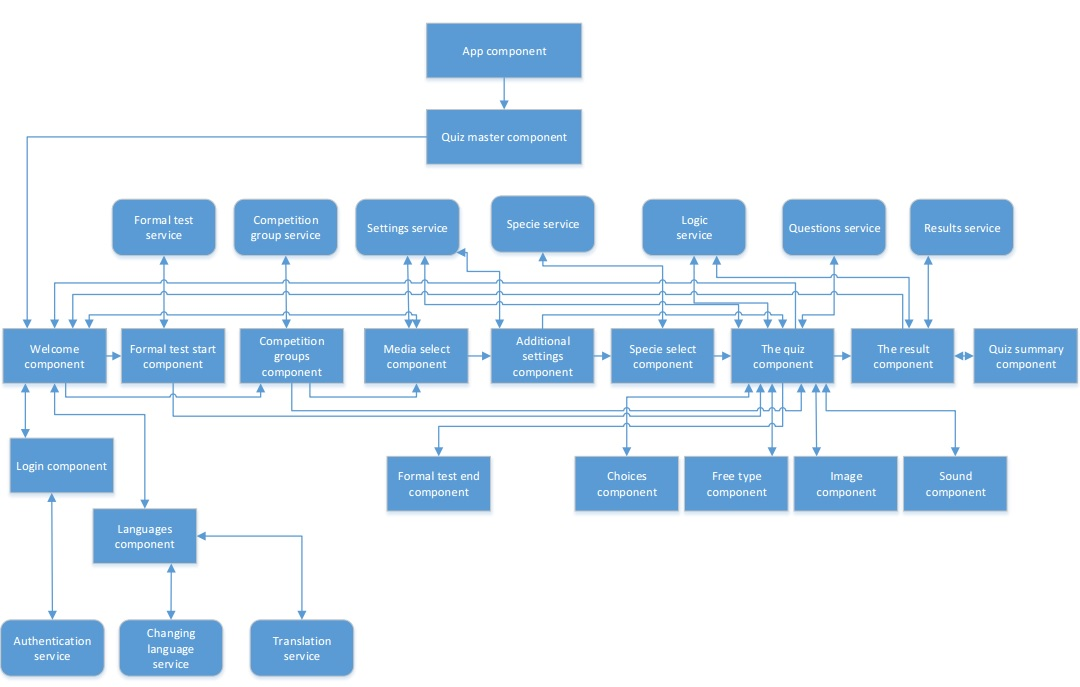
\includegraphics[width=1.0\textwidth]{figures/system_architecture.jpg}
  \caption[Hierarchy]{System architecture}
  \label{fig:Hierarchy}
\end{figure}

Everything starts at the top with bootstrapping the main component, the app component. This component is only in charge of defining the routing for the application and then handing control over to its only child, the quiz master component. This is the boss/god of the application. Here all the services are started and initialized. The next thing to happen is that the loading graphics is replaced with the router outlet, defined in the parent, and the quiz app can start. It all then start at the beginning with the welcome component (not shown above) where the user can select between quiz, competition groups and formal test. Each of the next steps through a quiz uses the routing for switching the main component in focus and using services for both saving data between components and handling communication to the backed API.

Each normal quiz consist of several defined steps with one or more corresponding component. After selecting both the quiz and for example images then the user can input several additional parameter for he quiz like the area and difficulty level. These are defaulted to the most popular choice based on previous testing. All of these settings are then promptly saved in the quiz settings service which is all knowing about the state of the quiz, but does no processing or server communication. Then the quiz will start on the next step and the correct sub components will be loaded. For example the image component if an image quiz and the sound component if a sound quiz was chosen. Then the quiz question service retrieves a quiz from the API and sends it to the quiz logic service for processing. Each question is then contained in a quiz question objects which holds every peace of knowledge associated with that question. The reason for this is because later it can support  multiple questions in one (like in several sound quiz) with the rest of the application treats it as a single question. Once the quiz is over it will allow the user (if hints were not used) to submit score to server using the results service. Optionally, if they are logged in it will submit their results anyways for the user quiz statistic function on the server.

The formal test works a bit different. First off it requires an access code/token provided when your application is approved. Then the API does NOT return information about the choices and right answer to the question. It also does not return any usable media URL, just a one time token that can be exchanged once for the image. It also forces the users to do the free type where they have to select the correct specie from a list of all species. It also skips the in-between question part, giving no breaks. At the end it submits the response to the server, allowing examiners to grade the test. 

The last part in the competition group where people can compete inside a group with its own set of rules, limited amount of attempts, access codes and its own high score list. Can be used by anyone from friends to school classes. Once selected and clicked play it will go directly to the quiz with all settings stored if it has restrictions. Some groups have no restrictions, just having all high score submitted together. The login/authentication is entirely server side as client side security is no security. It offers the possibility of registering, login and resetting password. It also enables autologin and grating authenticating tokens and refresh tokens. There are some more features like  changing language, bit that is mostly self explanatory. 
%shall we mention that the group does not neccecary need to have pre defined settings?


The backend API will not be thoroughly documented as it is make mostly outside the scope of this project and it is not open source. Some documentation will be provided however, for example the API endpoints used by the quiz. The back-end is written in PHP 7 and is using MySQL. Most of the functionality used by the quiz already existed at the beginning of the project, at the already existing flash application but was using XML, not JSON. This was a problem since Angular 2 really favours JSON and it been more lightweight, as well as easier to work with in JavaScript/TypeScript. Some additional API's were added, for example the competition group listing. Throughout the development process some bugs were discovered in the old API  and were fixed, resulting  the already existent API benefiting from this project as well. 


\section{Strength and weaknesses of chosen technologies}
\label{sec:stregthandwic}
Most, if not all of the chosen technologies for this projects is cutting edge and some, like Angular 2 just being  barely in realise candidate level at the end of the project. We debated a lot over the choice between Angular 1 and 2. It boiled down to either continuing on a dying platform with great documentation and extensive knowledge base across the Internet including blog post and problems solved on stack overflow or venturing into the new and unknown. Angular 2 did however has too many new and exiting functionality for us to pass it up and we quickly learned how much easier Angular 2 is to use than Angular 1. In retrospective it almost seems like Angular 1 is just a prototype for what to come. Using a tutorial on Udemy \cite{TheCo73:online} we managed quickly to learn the new framework and start working. The modular approach of the framework greatly benefited the team as each person could work on there own component in parallel with the rest.

When it comes to great web design it is not really a debate on which framework to use. Bootstrap is the way to go. We debate a bit about using the new Bootstrap 4, but as it only was in alpha. We felt it was a bit too new and unstable for our project and decided to use the latest Bootstrap 3 with great success. The framework/design template worked wonderfully for a group with no designer as it let us create relative amazing looking quiz with little effort. It also handles responsiveness amazingly which is a big part of making a quiz which both work on desktop, tablets and mobile.

We also selected Sass\cite{Sass:14:online} over CSS for extra functionality, even if we did not really use all of it. If offers a lot of extra functionality not provided by plan old CSS, but is is just extending like TypeScript is extending JavaScript. It means we could always fall back on CSS if we did not know the correct Sass way of doing something. 

Another important choice was choosing Gulp for our automation tool as our previous automation tool as Grunt seemed to be dying. As a side note we do not really believe that gulp will live long either, but there is not greater tool right now. It is really easy to learn (and drop lather) offering most required functionality via plug-ins made by the community.

Selecting so many new technologies at the same time made it a lot more challenging to get started as we had to learn every new technology at the same time in parallel. This was one of the reasons we used a test repository the first sprint to test and learn everything before moving onto the real repository. Might be worth mentioning we used git and GitHub for version control as both greatly improve collaboration on coding projects, and makes it easier to blame the right person when it breaks.

\section{Alternative technical solutions}
\label{sec:alttec}

There are a lot of great alternatives to what we have chosen for this project. The choices was mostly in front-end since the back-end was already developed. The most important, Angular 2 could have been replaced with Angular 1, but it is a inferior framework. Angular 2 is improved on every area as well as somewhat forcing (or strongly encroaching) the use of TypeScript. All team members used Angular 1 in the last semester's project and all of us see a clean benefit with Angular 2. Other choices was jQuery and React, but both of them have the downside of just adding some JavaScript to the HTML documents, unlike Angular 2 which does it the other way around and take full control, for example jQuery is mostlly usefully for just adding some extra functionality to a website, not making a JavaScript application as Angular 2 is allowing us. React also has some great benefits, but it is rather strict in the sense that it can not be used for anything that can potentially compete  with Facebook, as they made it. We like no restrictions and therefore we dropped it, even if it can do a lot of amazing things.

%I guess decribe what angular 1 is and react + grunt and normal css?
\chapter{Conclusion}
\label{chap:conclusion}

%Conclusion goes here  (2-3 pages)
%\begin{itemize}
%\item Status of implementation – know limitations and weaknesses (functionality as well as
%technical solution)
%\item Reflection on project work (aka project retrospective)
%\item  Features that should be added in future versions of the application
%\item  Technical solutions that should be modified, replaced, or added in future version of
%the application; technologies that should be considered for future versions of the
%application
%\end{itemize}


\section{Status of implementation, limitations and weaknesses}
The quiz is completed as we originally intended. We planned for more features outside the quiz, but the core functionality was completed as intended. It was really great to actually complete what we planned, especially after falling really short on our plans last semester.However there is one exception to this, we never added the special area, but it was not clear  if it will ever be used. It works on many ways exactly the same as competition groups.

The current implementation is not perfect, as mentioned it lacks a bit in the testing department, both manual user testing and automatic scripted testing. We have not really had any problems from not having automatic testing bit we think we have now reached the point where any further work would require it.

\section{Reflection on project work}
(aka project retrospective)

We selected a wide range of new technologies for this project which contributed to a rather steep learning cure in the beginning as nobody really was familiar with anything. The first few weeks were therefore promptly spent learning everything so we could get to a point where we could start working. From there work speed steadily improved as our velocity chart should have shown if we had consistent length on sprints. We did however decide to focus more on always having something to do rather than sprints with fixed length and requiring all tasks to be done before the next. Development speed reached really high speed towards the end with 1/3 all commits being in the last sprint. This is due to most of them being really small and the team getting really familiar with the technologies. 

There was a real challenge in getting all team members working efficiently since we all did come from different backgrounds and learned in different ways. Despite some setbacks we did manage to get everyone to the same point by the end of the project. This type of experience with working on a initially divided team is really valuable as any team out in the real world will be like that at some point. Experiencing this diversity is very relevant experience that later on we can apply to a real job. The work was  structured as most program development projects with a focus on always learning something new and focusing on what benefits the user while using the latest in project organisation applications, like Jira.

%Angular 2 turned out to be the best

Working together at school was probably the best thing we did. The group dynamics was great where we in one moment was discussing a task and in the next debating the cultural differences. The social factor is just as important as being able to instantly discuss tasks as problems occur. Development time was clearly shorter when we worked together because it was much easier to explain tasks and challenges while visually showing what we where discussing. Remote only teams have some huge challenges here, especially getting each team member on the same page. For keeping a consistent vision of what the application/product is. We experienced how is it to work with some members of the team being away for a while. It is a valuable lesson learned on how the task should be clearly defined in Jira and how to communicate efficiently. 

In the beginning of the project the communication with the main supervisor was going really well, we had meetings and got valuable feedback and suggestions on the project but as the project progressed it became almost impossible to get a meting with the main supervisor.
At the end (last 3 sprints) we repeatedly asked for help with the project and we were turned down each time. This was the time when we need help the most. 
Is was fun, but we sort of miss help from main supervisor, at stage that he both abandoned us and took another group on a payed trip to Poland.

\section{Features to be added}
Even if the core quiz is ready we still have a lot of functionality we want to add in. The first in probably the special area where organisations can purchase a special area/page on the site with is own subset of species for a custom quiz. This might however be unnecessary as it really overlaps with competition groups. Only the future will tell what it will become in the end.

Another feature really requested is the video quiz where people can for example take a quiz showing videos of birds and then determining the specie of them. This will require a lot more storage that the sever currently have as videos are a lot larger then images and sounds. Some people prefer observing birds in more life like setting, as in the video. It will still just be one of many choices on how to take the quiz and the user own choice is till the most important.

The system currently has a hint system build in where the user can either remove choices or get the first letters of the specie name. This is just the start, we want to add even more ways of helping the user and giving them extra types of hints. One type of hints could be getting additional facts about the correct specie like its size, weight and wingspan. It could also be possible to click a button to get another image or sound of the specie to help identify it. The possibilities are almost endless.

Expanding on the last part about hints we would also want to further improve on the gamification elements in the system without harming the intrinsic motivation of the user to learn. This could be a really challenging task as adding gamification can easily destroy intrinsic motivation due to the over justification effect and may only work for a short time due to the novelty factor\cite{DoesG74:online}. There is great potential for improvement, but this is an merging field and we should tread carefully not to hurt what we already have. 

One potential problem with the system currently is that is requires manually inputting all the choices for any question somewhat manually. There is some automation, but the system could benefit by having mode where the choices/markers are automatically generated. This could be done by values already in the system like similar birds by appearance and sound. This could then  be used as a second difficulty to the media difficulty. Harder difficulties would have more similar choices. This could also be extended to hints by having a button that makes the choices easier. One problem with this kind of hints system however is that the user can just select the ones that does not change when asking for easier choices on the particular question.

The design and user experience of the current application need some improvements currently. A lot of functionality are not really self explanatory as well as not having the best design either. This is mostly due to no team member currently being a designer and what we made is more in the way of programmers design. Working, but far from perfect. One example is that the user can get overloaded with information in both additional settings and the actual quiz. For example, in the quiz there is an entire table showing all the quiz settings. This table should be either removed or completely redesigned. A solution is hiding it by default, but allowing users to see it by clicking a button like "show quiz settings". Another issue is how the list of available languages are in English, making it hard to select your own language if you do not know it in English, somewhat defeating the purpose of having a language select. Another problem regarding the area list as it is always in English no mater the active language. Most of these problems, if not all  should be possible to fix with further development testing and designing. 


\section{Technical solutions that should be improved}

The current build proses during development is entirely automatic using Gulp and lite server with node package manager (npm) for package management. However it is not perfect when it comes to deployment. It does not concatenate any files and requires the upload of all individual compiled files including all node dependencies. It is entirely possible to both concatenate all node dependencies and project files into one or two files of needed (for each file type like CSS and JS). We did not have time to implement this, but would really like to do this if we had the time. It would enormously speed up deployment and speed up application speed with less to transfer and load.

The system currently pulls all translation when it starts up. This can be significantly improved by doing local caching using local storage or indexed DB. It could fetch the translations the first time the app runs and then just ask for changes from the server. This could decrease load on the sever and amount of data transmitted, but not really improve app load time. This is due to a lot of other simultaneously server request are preformed on start up anyway. Some of these can be cached like the list of areas, but still competition groups needs to be loaded as well as the specie list and language list. All of these could also be cached, but just checking for changes is usually just as consuming time wise as just getting all the data. Also storing that much data on mobile devices will eat away from already really precious storage.

The project is in need of some cleanup and refactoring. Some services are fragmented and should be combined into one like change language service and translation puller. They are overlapping a lot and would greatly benefit from merging into one. This project has been developed in an iterative approach which led to a lot of unused code as new features were added. This should be cleaned up and maybe refactored in order to keep the project tidy and neat for further development. This project will most likely have a long lifespan with with the customer and having the code at its best for as long as possible will greatly help us in the future.

% \chapter{Packages}
\label{chap:packages}

The \texttt{gucthesis} is built upon the standard \LaTeX\
\texttt{report} class. All commands from the \texttt{report} class can
be used, with the two exceptions of \verb+\subsubsection+ and
\verb+\paragraph+. This is because there should only be three
levels of headings according to the guidelines~\cite{GUCMaster}.

\section{Packages Used by gucthesis}
\label{sec:packages}

In addition to the \texttt{report} document class,
\texttt{gucthesis} makes direct use of the following packages
that must hence be present:
\begin{description}
	\item[geometry:] used for setting the sizes of the margins and
  	headers.
	\item[fontenc:] used with option \texttt{T1} for forcing the Cork font
  	encoding (necessary for the Charter font).
	\item[charter:] load Charter as the default font.
	\item[euler:] load the Euler math fonts.
	\item[bable:] for language handling.
\end{description}

\section{Other Relevant Packages}
\label{sec:otherpackages}

The author of a thesis might want to use a bunch of different packages
to those described in Section~\ref{sec:packages} in order to have all features needed for their document. 
In particular, it is advised to use the following:
\begin{description}
	\item[inputenc:] to allow \LaTeX\ to use more than 7-bit ASCII for its
	  input. Most often, the option \texttt{latin1} will do.
	\item[babel:] to load language specific strings. Reasonable options
	  include \texttt{british}, \texttt{american}, \texttt{norsk} and
	  \texttt{nynorsk}.
	\item[graphicx:] to include graphics.
	\item[hyperref:] this is a very nice package that makes cross links in
	  pdf documents. Use with option \texttt{dvips} or \texttt{pdftex}
	  in accordance with the driver that you use. Unfortunately, hyperref
	  is not completely bugfree\dots
\end{description}




\bibliographystyle{gucthesis}
\bibliography{MastersExample}
%\begin{thebibliography}{9}
%\bibitem{RESTRef} 
%Fielding, Roy Thomas. \textit{Architectural Styles and the Design of Network-based Software Architectures}. Doctoral dissertation, University of California, Irvine, 2000
%\end{thebibliography}


%\end{gather*}

\appendix
\include{appendix}

\end{document}
